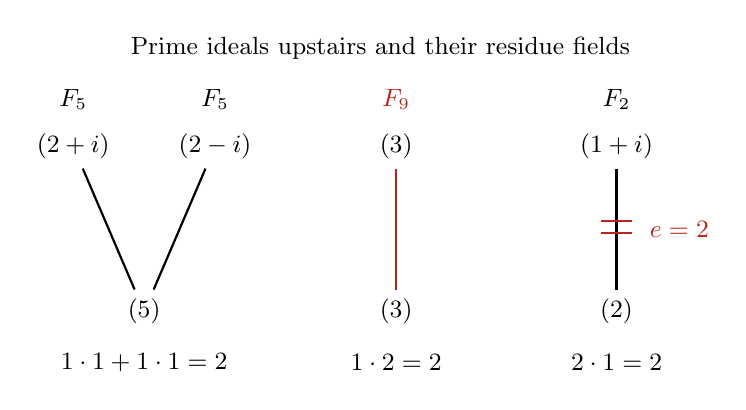
\begin{tikzpicture}[font=\small,x=1cm,y=1cm]
\node (p5) at (0,0) {$(5)$};
\node (a) at (-0.9,2.1) {$(2+i)$};
\node (b) at (0.9,2.1) {$(2-i)$};
\draw[thick] (p5)--(a);\draw[thick] (p5)--(b);
\node[above] at (-0.9,2.45) {$\mathbb F_5$};
\node[above] at (0.9,2.45) {$\mathbb F_5$};
\node at (0,-0.65) {$1\cdot1+1\cdot1=2$};
\node (p3) at (3.2,0) {$(3)$};
\node (c) at (3.2,2.1) {$(3)$};
\draw[thick,BrickRed] (p3)--(c);
\node[above,BrickRed] at (3.2,2.45) {$\mathbb F_9$};
\node at (3.2,-0.65) {$1\cdot2=2$};
\node (p2) at (6.0,0) {$(2)$};
\node (d) at (6.0,2.1) {$(1+i)$};
\draw[thick] (p2)--(d);
\draw[BrickRed,thick] (5.8,1.0)--(6.2,1.0);
\draw[BrickRed,thick] (5.8,1.15)--(6.2,1.15);
\node[right,BrickRed] at (6.3,1.05) {$e=2$};
\node[above] at (6.0,2.45) {$\mathbb F_2$};
\node at (6,-0.65) {$2\cdot1=2$};
\node at (3.0,3.35) {Prime ideals upstairs and their residue fields};
\end{tikzpicture}
